% ============================================================
% TD progressif : La loi normale -- cinq situations de terrain (2 h)
% Pôle Formation UIMM - CVDL - BTS Industriel - S. JAUBERT
% A traiter avant la suite du TD v2. Corrigé : MOD08_Loi_Normale_TD_Progressif_Corrige_v1_0
% ============================================================
\documentclass[a4paper,11pt]{article}
% Préambule commun TD / corrigé -- MOD08 Loi normale, TD progressif v1_0
\usepackage[utf8]{inputenc}
\usepackage[T1]{fontenc}
% babel-french absent sur certains postes : chargement conditionnel
\IfFileExists{french.ldf}{\usepackage[french]{babel}}{}
\usepackage{helvet}
\usepackage{courier}
\renewcommand{\familydefault}{\sfdefault}
\usepackage[top=3cm, bottom=2.5cm, left=2cm, right=2cm, headheight=2cm]{geometry}
\usepackage{amsmath,amssymb,amsfonts}
\usepackage{graphicx}
\usepackage[dvipsnames,table]{xcolor}
\usepackage{tikz}
\usetikzlibrary{patterns}
\usepackage[most]{tcolorbox}
\usepackage{fancyhdr}
\usepackage{enumitem}
\usepackage{array,needspace,booktabs}
\usepackage{titlesec}
\usepackage{hyperref}

\definecolor{uimmblue}{HTML}{005C85}
\definecolor{uimmred}{HTML}{D31326}
\definecolor{uimmlightblue}{HTML}{E8F1F8}
\definecolor{uimmgray}{HTML}{333333}
\definecolor{uimmlightgray}{HTML}{F5F5F5}
\hypersetup{colorlinks=true, linkcolor=uimmblue, urlcolor=uimmblue}

\titleformat{\section}{\Large\bfseries\color{uimmblue}}{}{0pt}{}[\vspace{2pt}{\color{uimmblue}\titlerule[1.2pt]}]
\titleformat{\subsection}{\large\bfseries\color{uimmblue}}{}{0pt}{}
\setlist[enumerate,1]{label={\color{uimmblue}\textbf{\arabic*.}}, leftmargin=*}
\setlist[enumerate,2]{label=\alph*), leftmargin=*}
\setlist[itemize,1]{label={\color{uimmblue}\textbullet}}

\newtcolorbox{exo}[1]{colback=white, colframe=uimmblue, fonttitle=\bfseries\color{white},
  coltitle=white, title={#1}, boxrule=1pt, arc=2pt,
  left=8pt, right=8pt, top=5pt, bottom=6pt, before skip=10pt, after skip=6pt}
\newtcolorbox{consigne}{colback=uimmlightgray, colframe=uimmgray, boxrule=0.8pt, arc=3pt,
  left=8pt, right=8pt, top=6pt, bottom=6pt}
\newtcolorbox{rappel}[1]{colback=uimmlightblue, colframe=uimmblue, fonttitle=\bfseries\color{white},
  coltitle=white, title={#1}, boxrule=0.8pt, arc=2pt,
  left=8pt, right=8pt, top=3pt, bottom=3pt, before skip=6pt, after skip=5pt, fontupper=\small}

\newcommand{\calc}{\,{\color{uimmred}\small\textbf{[calculatrice]}}}
\newcommand{\sanscalc}{\,{\color{uimmred}\small\textbf{[sans calculatrice]}}}
\newcommand{\duree}[1]{\hfill{\normalsize\color{uimmred}#1}}
% Zone de réponse lignée : #1 = nombre de lignes
\newcommand{\zone}[1]{\par\smallskip\noindent\begin{tikzpicture}
  \foreach \i in {1,...,#1}{\draw[uimmgray!30] (0,-0.74*\i) -- (\linewidth-1pt,-0.74*\i);}
  \end{tikzpicture}\par\smallskip}
\newcommand{\EnTete}[1]{%
\pagestyle{fancy}\fancyhf{}\renewcommand{\headrulewidth}{0pt}
\fancyhead[L]{\raisebox{-0.5\height}{
\includegraphics[height=1.5cm]{logo_uimm_placeholder.jpg}}}
\fancyhead[C]{\begin{minipage}{8cm}\centering
  {\small\color{uimmblue}\textbf{Pôle Formation UIMM - CVDL}}\\
  {\footnotesize\color{uimmgray} BTS Industriel -- Mathématiques}\end{minipage}}
\fancyhead[R]{{\small\color{uimmblue}\textbf{MOD08 -- #1}}}
\fancyfoot[C]{{\color{uimmblue}\rule{\textwidth}{1pt}}\\[2pt]
  {\footnotesize\color{uimmgray} Pôle Formation UIMM -- Centre-Val de Loire \hfill S. JAUBERT \hfill \thepage}}}
% Cloche : #1 = facteur d'échelle horizontal, #2 = hauteur
\newcommand{\cloche}[2]{\draw[uimmblue, thick, domain=-3.6:3.6, samples=80, smooth]
  plot ({#1*\x},{#2*exp(-\x*\x/2)});\draw[uimmgray] ({-3.8*#1},0) -- ({3.8*#1},0);}
\EnTete{TD progressif}

\begin{document}

\begin{tcolorbox}[colback=uimmblue, colframe=uimmblue, sharp corners, boxrule=0pt,
  left=14pt, right=14pt, top=8pt, bottom=8pt]
{\color{white}\LARGE\bfseries Travaux Dirigés -- MOD08}\\[4pt]
{\color{white}\large La loi normale~: TD progressif, cinq situations de terrain \hfill 2 h}
\end{tcolorbox}

\vspace{-2pt}
\noindent\small\begin{tabular}{@{}>{\bfseries\color{uimmblue}}l@{\hspace{10pt}}p{13.4cm}@{}}
Séquence~: & [S02] Variables aléatoires et lois usuelles \\
Compétences~: & [C04] calcul de probabilités (loi normale) \quad [C05] espérance, écart-type \\
Prérequis~: & cours MOD08 \textit{Loi normale}, sections 3 et 4 \\
Consignes~: & écrire la probabilité cherchée avec la variable aléatoire \textbf{avant} tout calcul. Probabilités arrondies à $10^{-4}$. Un réglage ou un seuil s'arrondit \textbf{dans le sens qui respecte l'exigence}. \\
\end{tabular}\normalsize

\begin{rappel}{L'essentiel~: 1. Lire une loi normale $\mathcal{N}(\mu\,;\sigma)$}
\begin{minipage}{0.47\linewidth}
$\mu$ est la \textbf{moyenne}~: le centre de la cloche.\\
$\sigma$ est l'\textbf{écart-type}~: la largeur de la cloche.\\
L'aire totale sous la cloche vaut $1$.\\
Une probabilité est une \textbf{aire}.\\[4pt]
La cloche est \textbf{symétrique} autour de $\mu$~:\\
$P(X \leq \mu) = P(X \geq \mu) = 0{,}5$.\\[4pt]
Règle des \textbf{68 -- 95 -- 99,7}~: entre $\mu - k\sigma$ et $\mu + k\sigma$ se trouvent environ $68\,\%$ ($k=1$), $95\,\%$ ($k=2$) et $99{,}7\,\%$ ($k=3$) des valeurs.
\end{minipage}\hfill
\begin{minipage}{0.5\linewidth}\centering
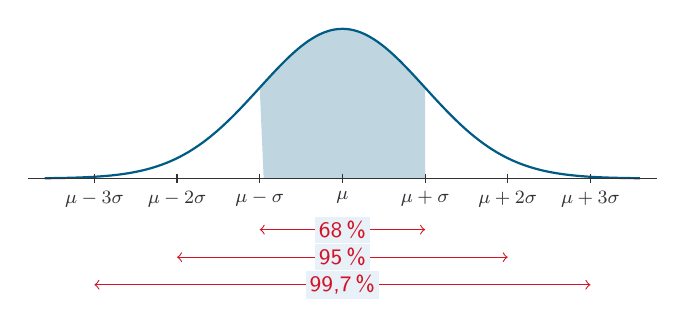
\begin{tikzpicture}[font=\footnotesize]
\fill[uimmblue!25, domain=-1:1, samples=40, smooth] (-1,0) -- plot ({1.05*\x},{1.9*exp(-\x*\x/2)}) -- (1.05,0) -- cycle;
\cloche{1.05}{1.9}
\foreach \k/\l in {-3/{\mu-3\sigma},-2/{\mu-2\sigma},-1/{\mu-\sigma},0/{\mu},1/{\mu+\sigma},2/{\mu+2\sigma},3/{\mu+3\sigma}}
  {\draw[uimmgray] ({1.05*\k},0.06) -- ({1.05*\k},-0.06) node[below, scale=0.85]{$\l$};}
\foreach \k/\y/\t in {1/-0.65/{68\,\%},2/-1.0/{95\,\%},3/-1.35/{99{,}7\,\%}}
  {\draw[uimmred, <->] ({-1.05*\k},\y) -- node[fill=uimmlightblue, inner sep=1.5pt]{\t} ({1.05*\k},\y);}
\end{tikzpicture}
\end{minipage}
\end{rappel}

\begin{rappel}{L'essentiel~: 2. Calculer une probabilité}
\textbf{À la calculatrice}, avec les vraies valeurs de $\mu$ et $\sigma$~:
\par\smallskip{\centering\footnotesize
\renewcommand{\arraystretch}{1.1}
\begin{tabular}{@{}lll@{}}
\toprule
 & \textbf{TI}~: \texttt{normalFRép(}borne inf, borne sup, $\mu$, $\sigma$\texttt{)} & \textbf{Casio}~: \texttt{Ncd} (Lower, Upper, $\sigma$, $\mu$) \\
\midrule
$P(a \leq X \leq b)$ & bornes $a$ et $b$ & Lower $=a$, Upper $=b$ \\
$P(X \leq b)$ & bornes $-10^{99}$ et $b$ & Lower $=-10^{99}$, Upper $=b$ \\
$P(X \geq a)$ & bornes $a$ et $10^{99}$ & Lower $=a$, Upper $=10^{99}$ \\
\bottomrule
\end{tabular}\par}\smallskip
\textbf{Passage à la loi centrée réduite.} Si $X \sim \mathcal{N}(\mu\,;\sigma)$, alors
\[
Z = \frac{X - \mu}{\sigma} \sim \mathcal{N}(0\,;1) \qquad\text{et}\qquad
P(X \leq x) = P\!\left(Z \leq \frac{x - \mu}{\sigma}\right).
\]
Le nombre $z = \dfrac{x-\mu}{\sigma}$ compte \textbf{à combien d'écarts-types} la valeur $x$ se trouve de la moyenne.\\[3pt]
\textit{Exemple.} $X \sim \mathcal{N}(50\,;4)$ et $x = 56$~: $z = \dfrac{56-50}{4} = 1{,}5$. Donc $P(X \leq 56) = P(Z \leq 1{,}5) \approx 0{,}9332$.
\end{rappel}

\begin{rappel}{L'essentiel~: 3. Le problème inverse~: on connaît la probabilité, on cherche la valeur}
\begin{itemize}[leftmargin=12pt, itemsep=3pt, topsep=2pt]
  \item \textbf{Chercher un seuil $x$} tel que $P(X \leq x) = p$~: \texttt{FracNormale($p$, $\mu$, $\sigma$)} (TI) ou \texttt{InvN} (Casio, Area $=p$).\\
  Même résultat avec la loi centrée réduite~: $x = \mu + z_p\,\sigma$, où $z_p = \texttt{FracNormale}(p)$.
  \item {\color{uimmred}\textbf{Attention.}} La calculatrice attend l'aire \textbf{à gauche} du seuil. Si l'énoncé donne l'aire à droite, $P(X \geq x) = p$, on entre $1 - p$. Toujours faire un schéma de la cloche.
  \item \textbf{Chercher $\mu$ ou $\sigma$}~: la calculatrice ne le fait pas directement. On écrit $\dfrac{x - \mu}{\sigma} = z_p$ et on résout l'équation.
\end{itemize}
\begin{center}\small
\renewcommand{\arraystretch}{1.2}
\begin{tabular}{|l|*{6}{c|}}\hline
Aire à gauche $p$ & $0{,}90$ & $0{,}95$ & $0{,}975$ & $0{,}99$ & $0{,}995$ & $0{,}999$ \\ \hline
$z_p$ & $1{,}2816$ & $1{,}6449$ & $1{,}9600$ & $2{,}3263$ & $2{,}5758$ & $3{,}0902$ \\ \hline
\end{tabular}\\[3pt]
Par symétrie, pour une aire à gauche $1-p$, la valeur est $-z_p$. Exemple~: $z_{0{,}05} = -1{,}6449$.
\end{center}
\end{rappel}

% ============================================================
\newpage
\subsection{Exercice 1 -- Débit d'entretoises~: lire la cloche \duree{Production -- [C04] [C05] -- 20 min}}

\begin{exo}{Contexte}
Une scie automatique débite des entretoises en aluminium. La longueur $L$ d'une entretoise, en mm, suit la loi normale $\mathcal{N}(120{,}00\,;0{,}05)$. Le plan impose $120{,}00 \pm 0{,}10$ mm.
\end{exo}

\begin{enumerate}
  \item Sous chaque graduation de la cloche, écrire la longueur correspondante, de $\mu - 3\sigma$ à $\mu + 3\sigma$. Hachurer la zone des entretoises conformes.
  \begin{center}
  \begin{tikzpicture}
  \cloche{1.7}{2.6}
  \foreach \k in {-3,...,3}{\draw[uimmgray] ({1.7*\k},0.08) -- ({1.7*\k},-0.08);
    \draw[uimmgray!50, densely dotted] ({1.7*\k-0.7},-0.25) rectangle ({1.7*\k+0.7},-0.85);}
  \draw[uimmgray!40, dashed] (0,0) -- (0,2.6);
  \end{tikzpicture}
  \end{center}
  \item \sanscalc{} Avec la règle des 68 -- 95 -- 99,7, donner une valeur approchée de~:
  \begin{enumerate}
    \item $P(119{,}95 \leq L \leq 120{,}05)$~;
    \item la probabilité qu'une entretoise soit conforme~;
    \item $P(L > 120{,}10)$. Justifier avec la symétrie de la cloche.
  \end{enumerate}
  \zone{3}
  \item \calc{} Calculer $P(119{,}90 \leq L \leq 120{,}10)$ et $P(L < 119{,}90)$. Comparer avec la question 2.
  \zone{3}
  \item La scie débite $4\,000$ entretoises par poste. Combien d'entretoises non conformes attend-on en moyenne par poste~?
  \zone{2}
  \item Un opérateur mesure une entretoise à $120{,}13$ mm.
  \begin{enumerate}
    \item À combien d'écarts-types de la moyenne cette mesure se trouve-t-elle~?
    \item Calculer $P(L > 120{,}13)$.
    \item Cette mesure doit-elle alerter l'opérateur~? Argumenter.
  \end{enumerate}
  \zone{4}
\end{enumerate}

% ============================================================
\newpage
\subsection{Exercice 2 -- Roulements de convoyeurs \duree{Maintenance -- [C04] [C05] -- 20 min}}

\begin{exo}{Contexte}
Un site logistique exploite $40$ convoyeurs à bande. Chaque motoréducteur est équipé d'un roulement du fournisseur A. La durée de vie $T$ d'un roulement, en heures de fonctionnement, suit la loi normale $\mathcal{N}(18\,000\,;2\,000)$.

Le service maintenance remplace tous les roulements, à titre préventif, à $15\,000$ h.
\end{exo}

\begin{enumerate}
  \item Calculer la probabilité qu'un roulement casse avant le remplacement préventif, c'est-à-dire avant $15\,000$ h.
  \zone{3}
  \item Sans remplacement préventif, quelle serait la probabilité qu'un roulement dépasse $20\,000$ h~?
  \zone{3}
  \item Calculer $P(16\,000 \leq T \leq 21\,000)$.
  \zone{3}
  \item Sur les $40$ roulements du site, combien cassent en moyenne avant $15\,000$ h~?
  \zone{2}
  \item Un fournisseur B propose, au même prix, des roulements dont la durée de vie $T_B$ suit la loi normale $\mathcal{N}(17\,000\,;1\,000)$.
  \begin{enumerate}
    \item Calculer $P(T_B < 15\,000)$.
    \item Un technicien affirme~: «~Les roulements A durent plus longtemps en moyenne, donc il faut garder A.~» Que lui répondre~?
  \end{enumerate}
  \zone{6}
\end{enumerate}

% ============================================================
\newpage
\subsection{Exercice 3 -- Précision d'un robot d'insertion \duree{Robotique -- [C04] -- 25 min}}

\begin{exo}{Contexte}
Dans une cellule robotisée, un robot 6 axes insère des goupilles dans un carter. On note $X$ l'écart, en mm, entre la position visée et la position atteinte. À froid, $X$ suit la loi normale $\mathcal{N}(0\,;0{,}02)$.

L'insertion réussit si $-0{,}05 \leq X \leq 0{,}05$. Sinon, la cellule s'arrête en défaut.
\end{exo}

\begin{enumerate}
  \item Calculer la probabilité qu'une insertion réussisse.
  \zone{2}
  \item Le robot réalise $2\,400$ insertions par poste. Combien d'arrêts en défaut attend-on en moyenne par poste~?
  \zone{2}
  \item En fin de poste, l'échauffement des axes décale le robot~: $X$ suit alors la loi $\mathcal{N}(0{,}01\,;0{,}02)$.
  \begin{enumerate}
    \item Calculer la nouvelle probabilité de réussite.
    \item Combien d'arrêts attend-on pour $2\,400$ insertions dans ces conditions~? Commenter l'effet d'un décalage de $10$ micromètres.
  \end{enumerate}
  \zone{5}
  \item On revient au robot à froid~: $X \sim \mathcal{N}(0\,;0{,}02)$.
  \begin{enumerate}
    \item Déterminer le réel $a$ tel que $P(X \leq a) = 0{,}95$. Arrondir à $10^{-3}$ mm.
    \item On cherche $h > 0$ tel que $P(-h \leq X \leq h) = 0{,}99$. Faire un schéma de la cloche. Quelle est l'aire à gauche de $h$~? En déduire $h$, arrondi à $10^{-3}$ mm.
    \item Le fabricant annonce~: «~$99\,\%$ des poses sont à moins de $0{,}05$ mm de la cible.~» Cette annonce est-elle exacte~?
  \end{enumerate}
  \zone{8}
\end{enumerate}

% ============================================================
\newpage
\subsection{Exercice 4 -- Couple de serrage d'une visseuse \duree{Production -- [C04] [C05] -- 25 min}}

\begin{exo}{Contexte}
Sur une ligne d'assemblage, une visseuse électrique serre les vis de fixation d'un carter. Le couple de serrage $C$, en N$\cdot$m, suit la loi normale $\mathcal{N}(\mu\,;0{,}4)$. Le réglage actuel est $\mu = 25{,}0$.

Un vissage est conforme si $24{,}0 \leq C \leq 26{,}2$. En dessous de $24{,}0$, la vis risque de se desserrer. Au-dessus de $26{,}2$, le filetage risque d'être endommagé.
\end{exo}

\begin{enumerate}
  \item Calculer $P(C < 24{,}0)$, $P(C > 26{,}2)$, puis la proportion de vissages conformes.
  \zone{4}
  \item Déterminer le couple $c_1$ dépassé par $99\,\%$ des vissages. Arrondir à $10^{-2}$ N$\cdot$m.
  \zone{4}
  \item Le client exige que la proportion de vissages sous $24{,}0$ N$\cdot$m ne dépasse pas $0{,}1\,\%$. Le régleur ne peut agir que sur $\mu$. L'écart-type reste égal à $0{,}4$.
  \begin{enumerate}
    \item Traduire l'exigence du client par une inégalité portant sur $C$.
    \item Déterminer la valeur minimale de $\mu$. Arrondir à $10^{-2}$ N$\cdot$m dans le sens qui respecte l'exigence.
  \end{enumerate}
  \zone{7}
  \item Pour ce nouveau réglage, calculer $P(C > 26{,}2)$, puis la proportion totale de vissages non conformes. Comparer avec la question 1. Sur quel paramètre faudrait-il agir pour satisfaire le client sans dégrader la conformité~?
  \zone{5}
\end{enumerate}

% ============================================================
\newpage
\subsection{Exercice 5 -- Délai et prix d'un chantier \duree{Chargé d'affaires -- [C04] [C05] -- 30 min}}

\begin{exo}{Contexte}
Un chargé d'affaires chiffre l'installation d'une ligne de convoyage chez un client. D'après les chantiers comparables déjà réalisés par son entreprise~:
\begin{itemize}[leftmargin=12pt, itemsep=1pt, topsep=3pt]
  \item la durée $D$ du chantier, en jours ouvrés, suit la loi normale $\mathcal{N}(38\,;4)$~;
  \item le coût de revient $K$ du chantier, en euros, suit la loi normale $\mathcal{N}(120\,000\,;8\,000)$.
\end{itemize}
Le contrat prévoit des pénalités de retard si le délai annoncé est dépassé. L'affaire est perdante si le coût de revient dépasse le prix de vente.
\end{exo}

\begin{enumerate}
  \item Le client souhaite un délai de $40$ jours. Quelle est la probabilité de tenir ce délai~? Quel est le risque de payer des pénalités~?
  \zone{3}
  \item Quel délai le chargé d'affaires doit-il annoncer pour le tenir dans $95\,\%$ des cas~? Arrondir au jour entier dans le sens qui respecte l'objectif.
  \zone{3}
  \item Le chargé d'affaires envisage un prix de vente de $130\,000$~\texteuro. Calculer la probabilité que l'affaire soit perdante.
  \zone{2}
  \item La direction veut que la probabilité d'une affaire perdante ne dépasse pas $2\,\%$. Déterminer le prix de vente minimal. Arrondir à la centaine d'euros dans le sens qui respecte l'objectif.
  \zone{3}
  \item Le client impose finalement $42$ jours, et l'entreprise veut tenir ce délai dans $95\,\%$ des cas. La durée moyenne reste de $38$ jours.
  \begin{enumerate}
    \item Déterminer l'écart-type maximal de la durée du chantier. Arrondir à $10^{-1}$ jour dans le sens qui respecte l'objectif.
    \item Concrètement, que signifie «~réduire l'écart-type~» pour un chantier~? Citer deux actions possibles.
  \end{enumerate}
  \zone{5}
\end{enumerate}

\end{document}
